\chapter{Experiment}

\section{Experimental Setup}

\subsection{Data Split and Target}
We use a strict chronological split to avoid look-ahead bias:
\begin{itemize}
	\item Training years: 2019--2023
	\item Validation year: 2024
	\item Test year: 2025
\end{itemize}

The prediction target is 5-day ahead return \texttt{future\_ret\_5}.

\subsection{Input Features}
All models are trained on the same 15 engineered price/fundamental features to ensure fair comparison:
\begin{align*}
\{&\texttt{ret\_1},\texttt{ret\_5},\texttt{ret\_10},\texttt{ret\_20},\texttt{hl\_spread},\texttt{co\_ret},\texttt{log\_vol},\\
&\texttt{turnover\_rate},\texttt{volume\_ratio},\texttt{pb},\texttt{ma5\_gap},\texttt{ma10\_gap},\texttt{ma20\_gap},\\
&\texttt{volatility\_5},\texttt{volatility\_20}\}
\end{align*}

For sequence models (LSTM/GRU), the sequence length is 30 and features are normalized per sequence by max-abs scaling.

\subsection{Baselines and Metrics}
We evaluate five non-graph baselines:
\begin{itemize}
	\item Linear factor model: Ridge
	\item Nonlinear tabular models: LightGBM, XGBoost
	\item Deep temporal models: LSTM, GRU
\end{itemize}

Reported metrics include IC, RankIC, SignAcc, Sharpe, MSE, and cross-sectional Top-$k$ portfolio metrics (IRR/Sharpe).

\section{Main Results}

\begin{table}[htbp]
\centering
\caption{Test-set performance comparison (2025)}
\label{tab:main-test-results}
\begin{tabular}{lccc}
\hline
Model & Test IC & Test RankIC & Top10 Sharpe \\
\hline
Ridge & 0.03568435 & 0.00069723 & -- \\
LightGBM & 0.04974221 & 0.01374122 & 4.37949639 \\
XGBoost & 0.04866105 & 0.01128825 & 4.55806821 \\
LSTM & 0.02906183 & 0.02642975 & 2.55264244 \\
GRU & \textbf{0.05160307} & \textbf{0.04237023} & 4.41701568 \\
\hline
\end{tabular}
\end{table}

The results show two clear findings:
\begin{itemize}
	\item The 15 engineered price factors carry meaningful predictive signal across all model families.
	\item GRU and tree models form very strong non-graph baselines; GRU achieves the highest test IC, while XGBoost achieves the highest Top10 Sharpe.
\end{itemize}

\section{Model-by-Model Analysis}

\subsection{Tree Models: Strong and Stable}
Both LightGBM and XGBoost remain highly competitive:
\begin{itemize}
	\item LightGBM: Test IC $=0.04974221$, Top10 Sharpe $=4.3795$
	\item XGBoost: Test IC $=0.04866105$, Top10 Sharpe $=4.5581$
\end{itemize}
These two models are strong tabular baselines for the final comparison table.

\subsection{GRU: Best IC in This Round}
GRU delivers the strongest test IC among all five models:
\begin{itemize}
	\item Test IC $=0.05160307$
	\item Test RankIC $=0.04237023$
	\item Top10 Sharpe $=4.4170$
\end{itemize}
Therefore, under the current single-modality price-factor setting, GRU is at least on par with tree models and slightly better in IC.

\subsection{LSTM: Usable but Unstable}
LSTM is not completely ineffective, but it is unstable during training:
\begin{itemize}
	\item Best epoch appears at epoch 1
	\item Best validation IC $=0.05708638$
	\item Test IC $=0.02906183$
\end{itemize}
This suggests LSTM can capture some signal but quickly loses generalization after further optimization. In this task, GRU is better aligned than LSTM.

\subsection{Ridge: Important Linear Reference}
Ridge reaches Test IC $=0.03568435$, lower than nonlinear models but still clearly positive. This provides a robust linear multi-factor baseline and supports the value of nonlinear methods.

\section{Short-Horizon Target: Why \texttt{ret\_1} Looks Easier}

In a supplementary run, we also replace the 5-day return target with the 1-day return target \texttt{future\_ret\_1}. The main empirical observation is that the IC becomes higher, but this does not mean the model becomes fundamentally stronger. The prediction task itself is easier.

\subsection{Microstructure Effects Matter More at One Day}

One-day returns are more sensitive to local market microstructure, such as intraday sentiment, liquidity pressure, and order flow. These effects are easier for our engineered features to capture, especially volume-related variables and short-horizon price momentum. As a result, \texttt{ret\_1} is naturally more predictable than \texttt{ret\_5}.

\subsection{Longer Horizons Contain More Noise}

Five-day returns mix in more sources of uncertainty, including macro shocks, sector rotation, and random cross-sectional drift. This increases the noise level of the target. By contrast, one-day returns stay more local and more directly linked to the latest market state, so IC is easier to obtain.

\subsection{Higher IC Does Not Mean Less Overfitting}

The higher \texttt{ret\_1} IC should also be interpreted carefully. A model can achieve a better IC on a simpler short-horizon target while still overfitting short-term patterns. In practice, this is exactly what we observe: train IC remains much higher than validation and test IC, which means the model is still learning short-range structure rather than a fully robust alpha signal.

\subsection{Practical Implication}

This supplementary result is useful because it confirms that the feature set does contain short-horizon predictive information. However, the more important and harder setting is still \texttt{future\_ret\_5}, since it is closer to a realistic portfolio construction horizon and exposes whether the model can generalize beyond local market inertia.

For a concrete reference, the LightGBM run on \texttt{future\_ret\_1} with price and news features gives much stronger in-sample fit than the 5-day target, but the out-of-sample advantage is much smaller:
\begin{itemize}
\item Train IC $=0.29256246$, Val IC $=0.07432835$, Test IC $=0.06360294$
\item Train RankIC $=0.20117949$, Val RankIC $=0.03790694$, Test RankIC $=0.01461429$
\item Train Top10 Sharpe $=15.97407609$, Val Top10 Sharpe $=3.54472250$, Test Top10 Sharpe $=3.89395440$
\item Train Top30 Sharpe $=12.67766503$, Val Top30 Sharpe $=1.94790793$, Test Top30 Sharpe $=3.28545027$
\item Train Top50 Sharpe $=10.57799773$, Val Top50 Sharpe $=1.48605285$, Test Top50 Sharpe $=2.71897655$
\end{itemize}

This pattern is consistent with the previous explanation: \texttt{ret\_1} is easier to fit because it is more local and more sensitive to short-term microstructure, but it also makes overfitting more obvious. The gap between train IC and test IC is still large, so the higher score should be interpreted as a task simplification effect rather than a fundamentally more powerful model.

\section{Generalization Gap and Overfitting}

A noticeable train--validation/test gap remains. For example:
\begin{itemize}
	\item GRU: Train IC $=0.2479$, Val IC $=0.0203$, Test IC $=0.0516$
	\item LightGBM: Train IC $=0.3044$, Val IC $=0.0529$, Test IC $=0.0497$
\end{itemize}
This is consistent with the high-noise nature of short-horizon return prediction in equities. The gap should be acknowledged as a key limitation, but the positive out-of-sample IC confirms that useful signal still exists.

\section{Effect of News Features}

\subsection{Motivation: Why Supplement Price with News?}

Price-based factors capture historical market dynamics but fail to incorporate external information such as news events, which may affect short-term price movements. To assess whether news provides incremental predictive value and to understand how different model architectures utilize such event-driven information, we construct a multimodal experimental setup by augmenting the 15 price factors with 13 daily aggregated news features (28 in total).

The studied models are:
\begin{itemize}
\item LightGBM + price + news
\item XGBoost + price + news
\item GRU + price + news
\end{itemize}

We maintain the same chronological split (train 2019--2023, validation 2024, test 2025) and target \texttt{future\_ret\_5} as the price-only baseline to enable fair comparison.

\subsection{News Feature Construction}

Each raw news item is first scored by sentiment analysis, then aggregated by stock-date. The final news feature set includes:

\begin{itemize}
\item \textbf{Count features:} \texttt{news\_cnt\_1d}, \texttt{news\_cnt\_3d}, \texttt{news\_cnt\_7d}
\item \textbf{Sentiment features:} \texttt{news\_sent\_mean\_1d}, \texttt{news\_sent\_mean\_3d}, \texttt{news\_sent\_mean\_7d}
\item \textbf{Dispersion/extreme features:} \texttt{news\_sent\_std\_7d}, \texttt{news\_sent\_max\_3d}, \texttt{news\_sent\_min\_3d}
\item \textbf{Event polarity/risk features:} \texttt{news\_pos\_cnt\_3d}, \texttt{news\_neg\_cnt\_3d}, \texttt{news\_risk\_cnt\_7d}
\item \textbf{Recency indicator:} \texttt{days\_since\_last\_news}
\end{itemize}

To avoid look-ahead bias, all aggregated news features are shifted by one trading day before being used for prediction. This ensures that only information available at time $t$ is used to predict future returns at time $t+5$.

\subsection{Impact on Tree-Based Models}

Incorporating news features leads to consistent improvements in tree-based models. Table~\ref{tab:news-test-results} shows that LightGBM achieves the best overall performance, with modest gains in IC and more significant improvements in top-$k$ portfolio Sharpe ratios (Table~\ref{tab:news-vs-price-delta}).

The improvement is more pronounced in top-$k$ selection (e.g., Top30 and Top50), where LightGBM gains $\Delta$ Top30 Sharpe $= +0.6213$ and $\Delta$ Top50 Sharpe $= +0.3721$. In contrast, test IC improves by only $\Delta$ IC $= +0.00142$. XGBoost shows a similar pattern: nearly flat IC change ($+0.00008107$) but larger top-$k$ Sharpe gains. 

This indicates that news signals act as a \textbf{filtering mechanism that enhances stock selection} rather than a dominant predictive factor for overall ranking. Tree models can effectively combine price features and news signals to identify higher-conviction investment opportunities.

\subsection{Impact on Sequential Models}

In contrast, incorporating news features into the GRU model results in a noticeable performance degradation (Table~\ref{tab:news-vs-price-delta}). Test IC decreases by $\Delta$ IC $= -0.02468536$, and top-$k$ Sharpe ratios also decline significantly ($\Delta$ Top30 Sharpe $= -0.7100$). The model exhibits early overfitting and fails to generalize to the test set.

This suggests that the current representation of news features is fundamentally unsuitable for sequential modeling. Unlike price features, which exhibit smooth temporal dependencies, news signals are \textbf{sparse, event-driven, and irregular over time}. When concatenated as dense time series inputs, they introduce noise and hinder the learning of temporal patterns inherent to sequential models like GRU.

\subsection{Feature Importance Analysis}

To understand which features contribute most to predictions, we analyze feature importance in the LightGBM model. Figures~\ref{fig:importance-price-only} and~\ref{fig:importance-news-augmented} present the feature importance distributions for price-only and news-augmented LightGBM respectively.

\begin{figure}[htbp]
\centering
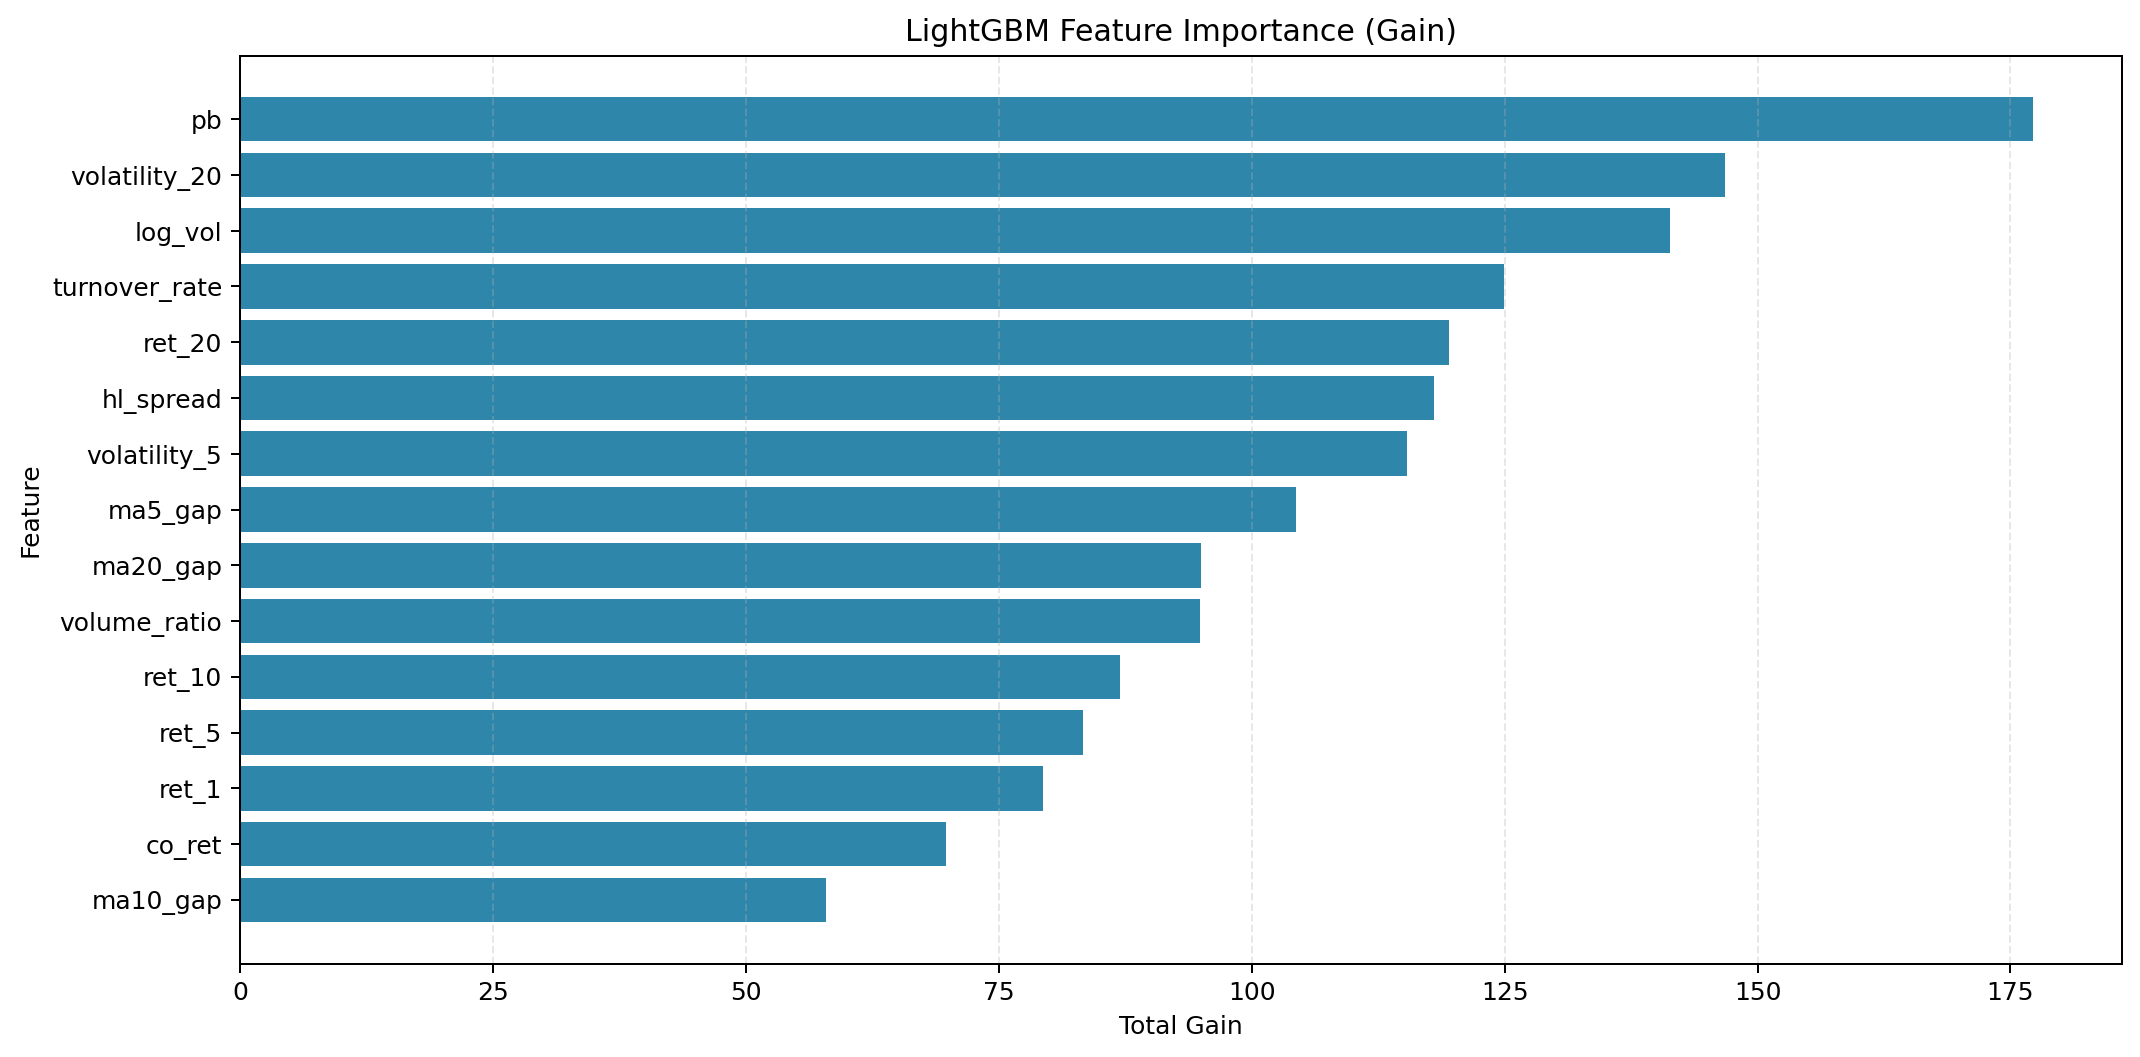
\includegraphics[width=0.95\textwidth]{experiment/feature_importance_gain_price_only.png}
\caption{Feature importance (by gain) for LightGBM trained on price factors only. Price-based features dominate, with \texttt{pb}, \texttt{volatility\_20}, and \texttt{log\_vol} ranking in the top 3.}
\label{fig:importance-price-only}
\end{figure}

\begin{figure}[htbp]
\centering
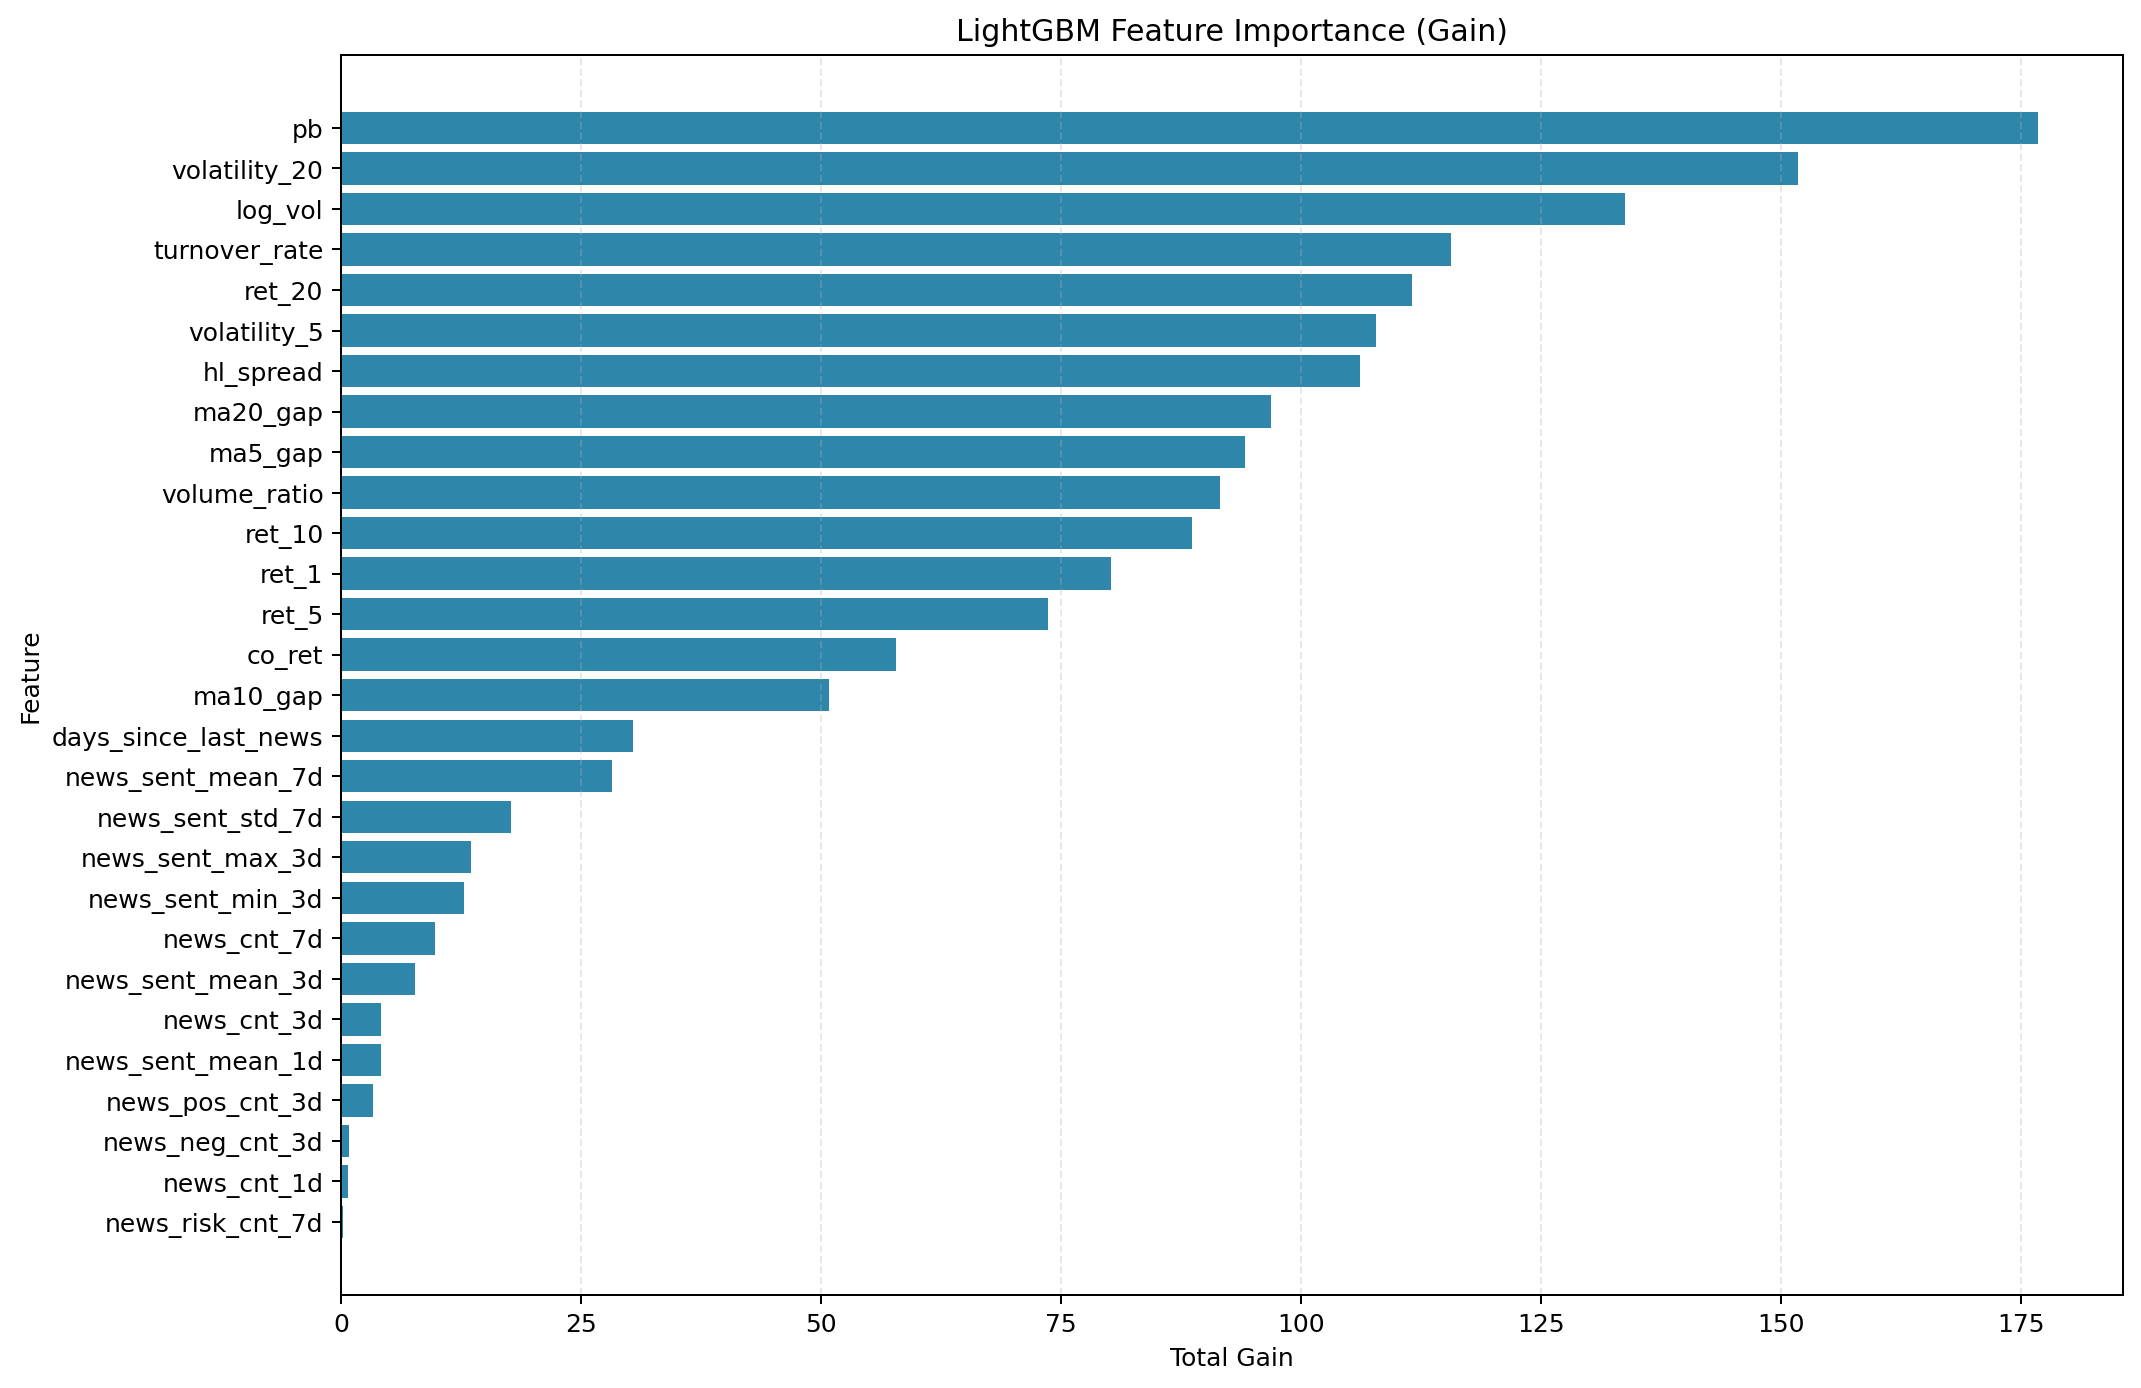
\includegraphics[width=0.95\textwidth]{experiment/feature_importance_gain_price_and_news.png}
\caption{Feature importance (by gain) for LightGBM trained on price and news factors. Price features remain dominant, but news-based features now appear in the ranking, with sentiment-related features (e.g., \texttt{news\_sent\_mean\_7d}) ranking higher than frequency-based features. The highest-ranked news feature (\texttt{days\_since\_last\_news}) is ranked 16th overall.}
\label{fig:importance-news-augmented}
\end{figure}

Key observations from the feature importance analysis are:

\begin{itemize}
\item \textbf{Price factors remain dominant.} In both the price-only and news-augmented models, price-based features occupy the top 15 rankings. \texttt{pb}, \texttt{volatility\_20}, and \texttt{log\_vol} are consistently ranked in the top 3, confirming that price factors capture the primary predictive signal.

\item \textbf{News features are actively utilized.} News features appear among the ranked features in the news-augmented model, indicating that LightGBM actively leverages news information during training. Notably, sentiment-based features (\texttt{news\_sent\_mean\_7d}, \texttt{news\_sent\_std\_7d}, \texttt{news\_sent\_max\_3d}) rank higher in importance than frequency-based features (\texttt{news\_cnt\_*}), suggesting that the \textbf{tone and distribution of news matter more than volume alone}.

\item \textbf{News serves as a complementary signal.} The improvement in top-$k$ selection without a corresponding improvement in overall IC confirms that news features provide targeted filtering rather than systematic ranking improvement. This aligns with the interpretation that news identifies regime shifts or high-impact events that affect subsets of stocks.

\end{itemize}

\subsection{Discussion and Interpretation}

The differential impact of news across model architectures reveals fundamental insights into how different models handle event-driven information:

\begin{enumerate}
\item \textbf{Event-driven vs.\ time-series representation.} News features are inherently event-driven and sparse, fundamentally different from traditional time-series features. Tree-based models excel at capturing such sparse and non-linear signals through their split-based decision structure, while sequential models struggle because they rely on smooth temporal dependencies.

\item \textbf{Model architecture determines information utilization.} The contrasting results for tree models (improvement) and GRU (degradation) demonstrate that model architecture is critical for leveraging multimodal information. Tree models treat each feature independently and can ignore noise, whereas RNNs attempt to learn temporal correlations among all inputs, making them sensitive to sparse noise.

\item \textbf{Implication for graph-based modeling.} These findings suggest that news information is better modeled through \textbf{relational and event-driven dependencies rather than as a time series}. This motivates the use of graph neural networks, which can explicitly represent event propagation, cross-stock relationships, and temporal event sequences in a structured manner.

\end{enumerate}

\subsection{Baseline Selection}

Compared with price-only baselines, incorporating news yields consistent but modest improvements in tree models, while degrading GRU performance. Therefore, under the current non-graph setting, \textbf{LightGBM + price + news} is selected as the strongest non-graph multimodal baseline for subsequent comparison with graph-based approaches.

\begin{table}[htbp]
\centering
\caption{News-enhanced model performance on 2025 test set}
\label{tab:news-test-results}
\begin{tabular}{lcccc}
\hline
Model & Test IC & Test RankIC & Top30 Sharpe & Top50 Sharpe \\
\hline
XGBoost + News & 0.04874212 & 0.01384341 & 4.61825196 & 4.54984642 \\
LightGBM + News & \textbf{0.05116316} & 0.01545951 & \textbf{4.84635056} & \textbf{4.72459068} \\
GRU + News & 0.02691771 & 0.01575878 & 3.29921022 & 2.99269869 \\
\hline
\end{tabular}
\end{table}

\begin{table}[htbp]
\centering
\caption{Change from price-only to price+news on test set}
\label{tab:news-vs-price-delta}
\begin{tabular}{lccc}
\hline
Model & $\Delta$ Test IC & $\Delta$ Top30 Sharpe & $\Delta$ Top50 Sharpe \\
\hline
XGBoost & +0.00008107 & +0.39023861 & +0.09317383 \\
LightGBM & +0.00142095 & +0.62126981 & +0.37211872 \\
GRU & -0.02468536 & -0.71000960 & -0.60178435 \\
\hline
\end{tabular}
\end{table}

\section{Effect of Policy Features}

\subsection{Two Policy Feature Construction Methods}

To further incorporate macro policy information, we implemented two different policy feature pipelines and compared them under the same LightGBM setup (train 2019--2023, validation 2024, test 2025).

\paragraph{Method A: Market-level policy aggregation}
In the first method, all policy documents are aggregated at the market level by date, without sector differentiation. Daily policy count and sentiment are rolled into 7-day and 30-day windows, producing:
\texttt{policy\_cnt\_7d}, \texttt{policy\_cnt\_30d}, \texttt{policy\_support\_score\_7d}, \texttt{policy\_support\_score\_30d}, and \texttt{days\_since\_last\_policy}.
These features are then merged to all stocks on the same date.

\paragraph{Method B: Sector-aware policy aggregation}
In the second method, each stock is mapped to a sector and policy records contain sector relevance weights. For a policy sentiment score $s$, sector weight $w$, and global policy sentiment mean $\mu$, we compute a sector-adjusted score
\[
s_{\text{adj}} = \mu + (s - \mu) \cdot w.
\]
Only positive sector-match weights are kept as effective signals. Then for each stock, sector-level policy signals are rolled over time into:
\texttt{policy\_7d}, \texttt{policy\_30d}, \texttt{policy\_cnt\_7d}, and \texttt{days\_since\_last\_policy}.
All policy features are shifted by one day to avoid leakage.
This design aims to convert policy information from a market-wide signal into a stock-specific sector-aware signal.

\subsection{Comparison Between the Two Policy Methods}

Table~\ref{tab:policy-method-comparison} reports the direct comparison. The old market-level method shows high in-sample fit but fails to generalize (negative test IC). The sector-aware method substantially improves robustness: validation IC remains modest, but test IC returns to a clear positive value and Top-$k$ Sharpe is strong.

\begin{table}[htbp]
\centering
\caption{Comparison of two policy feature construction methods (LightGBM + price + news + policy)}
\label{tab:policy-method-comparison}
\begin{tabular}{lcccc}
\hline
Method & Test IC & Test RankIC & Top30 Sharpe & Top50 Sharpe \\
\hline
Market-level policy aggregation (Method A) & -0.03577257 & -0.03729665 & 3.73783433 & 4.24234969 \\
Sector-aware policy aggregation (Method B) & 0.04646233 & 0.01076620 & 4.81798179 & 4.86964543 \\
\hline
\end{tabular}
\end{table}

This confirms that the sector-aware design is a meaningful correction over the earlier policy formulation. In other words, policy features are no longer ``dangerous'' enough to collapse out-of-sample IC, but become a controllable auxiliary signal.

\subsection{Feature Importance Comparison for Two Policy Methods}

We further compare feature importance distributions of the two policy methods in Figures~\ref{fig:importance-policy-method-a} and~\ref{fig:importance-policy-method-b}.

\begin{figure}[htbp]
\centering
\includegraphics[width=0.95\textwidth]{experiment/feature_importance_gain_policy.png}
\caption{Feature importance (gain) under Method A (market-level policy aggregation). Policy features dominate the top ranks, and this version exhibits poor out-of-sample IC.}
\label{fig:importance-policy-method-a}
\end{figure}

\begin{figure}[htbp]
\centering
\includegraphics[width=0.95\textwidth]{experiment/feature_importance_gain_sector.png}
\caption{Feature importance (gain) under Method B (sector-aware policy aggregation). Policy features are still strong, but the model generalization is substantially improved.}
\label{fig:importance-policy-method-b}
\end{figure}

Under Method B, policy features still occupy the top positions (e.g., \texttt{policy\_30d}, \texttt{days\_since\_last\_policy}, \texttt{policy\_7d}), indicating that policy signal remains very influential. This explains why the method improves Top-$k$ selection but does not consistently improve full cross-sectional ranking stability year by year.

\subsection{Comparison with the Best Previous Baseline}

Although Method B is a clear improvement over Method A, it does not consistently outperform the strongest previous baseline (LightGBM + price + news, without sector-policy features) in overall ranking quality:

\begin{itemize}
\item Best previous baseline (price + news): Test IC $\approx 0.0512$, Top30 Sharpe $\approx 4.846$, Top50 Sharpe $\approx 4.725$
\item Sector-policy version (price + news + sector-policy): Test IC $=0.0465$, Top30 Sharpe $=4.818$, Top50 Sharpe $=4.870$
\end{itemize}

Therefore, policy currently behaves more like a \textbf{top-$k$ filtering enhancer} than a robust \textbf{global ranking enhancer}. It can improve head-portfolio selection in some periods, but does not yet provide a stable IC uplift over the strongest price+news baseline.
This suggests that policy signals may be more regime-dependent and sparse than price and news features, which limits their ability to provide stable full-universe ranking improvement.

\subsection{Conclusion for Policy Experiments}

The policy experiment can be summarized as:
\begin{itemize}
\item Method A (market-level policy) is overfitted and unstable out-of-sample.
\item Method B (sector-aware policy) successfully fixes the major failure mode and restores positive test IC.
\item However, policy features are still relatively dominant and temporally unstable; gains are stronger in Top-$k$ selection than in full-universe ranking.
\item For the current report, \textbf{LightGBM + price + news} remains the strongest and most stable non-graph baseline, while \textbf{sector-aware policy} is a promising but not yet consistently superior extension.
\end{itemize}

\section{First GNN Baseline: GCN with Industry Graph}

After establishing strong non-graph baselines, we begin to test graph neural networks. This is the first GNN in the project, and it is intentionally price-only: there are no news or policy features in this version. The objective is to isolate the contribution of graph structure itself.

\subsection{How the Graph Is Built}

The graph is constructed from the industry mapping file \texttt{zz500\_stock\_sector\_map.txt}. Each stock is treated as a node, and an edge is created between two stocks if they belong to the same sector. In practice, this produces an industry adjacency matrix where stocks within the same sector are fully connected, including self-connections on the diagonal.

This graph is then converted into \texttt{edge\_index} for PyTorch Geometric, so that the GCN can perform message passing over industry-linked stocks.

\subsection{How the Dataset Is Built}

To separate dataset construction from model training, we first generate a graph dataset on disk. The pipeline reads the monthly parquet files under \texttt{dataset\_by\_month}, fixes a global stock order from the sector map, and then creates one daily snapshot per trading day.

Each snapshot contains:
\begin{itemize}
\item \texttt{x}: node feature matrix of size $N \times 15$
\item \texttt{y}: future return target
\item \texttt{mask}: valid-label indicator for each stock
\item \texttt{trade\_date}: the corresponding trading date
\end{itemize}

The split remains strictly chronological:
\begin{itemize}
\item Train: 2019--2023
\item Validation: 2024
\item Test: 2025
\end{itemize}

This ensures that the graph experiment follows exactly the same no-leakage protocol as the LightGBM and GRU baselines.

\subsection{GCN Design and Hyperparameters}

The model is a simple two-layer GCN:
\begin{itemize}
\item \texttt{GCNConv(15, 32)}
\item ReLU activation
\item Dropout disabled in the final stable run (\texttt{dropout = 0.0})
\item \texttt{GCNConv(32, 1)}
\end{itemize}

The final training configuration is:
\begin{itemize}
\item learning rate: \texttt{0.001}
\item weight decay: \texttt{1e-4}
\item early stopping patience: \texttt{20}
\item device: CUDA-only
\item best checkpoint selected by validation IC
\end{itemize}

We explicitly monitor validation IC after every epoch and keep the best model state. In our run, the best validation epoch is epoch 36, and the training stops at epoch 56 because validation IC no longer improves.

\subsection{Results}

The final GCN result on the 2025 test set is:
\begin{itemize}
\item Validation IC $=0.0692$
\item Test IC $=0.0561$
\item Test Top30 Sharpe $=4.1731$
\item Test Top50 Sharpe $=4.0833$
\end{itemize}

Compared with the price-only LightGBM baseline without news, which gives validation IC $=0.0529$, test IC $=0.0497$, Top30 Sharpe $=4.2251$, and Top50 Sharpe $=4.3525$, the GCN shows a clear improvement in IC-based ranking quality:
\begin{itemize}
\item Test IC: $0.0561 > 0.0497$
\item Validation IC: $0.0692 > 0.0529$
\end{itemize}

This is the key message of the first graph experiment: even without news or policy, the industry graph itself adds predictive value beyond price features. The GCN is therefore learning not only stock-level price patterns, but also the relational structure between stocks within the same sector.

At the same time, the head-portfolio metrics are still slightly weaker than LightGBM in this run:
\begin{itemize}
\item Top30 Sharpe: $4.1731 < 4.2251$
\item Top50 Sharpe: $4.0833 < 4.3525$
\end{itemize}

So the most accurate summary is that GCN improves global cross-sectional ranking quality, while LightGBM remains slightly stronger in some Top-$k$ portfolio metrics. This is still a strong result, because it shows that graph structure can contribute useful information even in a price-only setting.

\subsection{Takeaway}

This experiment gives a clean foundation for later graph-based work. It shows that a simple industry graph is already enough to beat the price-only LightGBM in IC, which justifies moving on to more advanced graph variants such as GAT, or to multimodal graph models that combine price, news, and policy information.
